\chapter{State of the Art}\label{section:state_of_the_art}

We will now depict the current state-of-the-art of what research is happening on the same topic in both economics and computer science.
Our goal will be to see if the state-of-the-art research presented hereunder does match the results that our simulation will yield.

\section{In economics}

Prof. Bayenet, Professor of ``Politique économique" (taught at ULB), presents economical politics as a domain of analysis and actions: governments (States) make some economical choices which orient the activity of agents. According to its slides \cite{bayenetSlides1}, the State has three major roles regarding economics:

\begin{itemize}
    \item \textbf{Allocation}: the State should correct the imperfections of the market and organize it. It should provide public goods and services if the market does not work properly
    \item \textbf{Stabilization}: the State should maintain the growth, limit inflation, aim at full employment, ... 
    \item \textbf{Redistribution}: the State should correct the inequalities in the distribution of wealth among its agents. This is the part we are the interested the most in. We have some leverage on this part thanks to the taxes that a State collects in order to distribute wealth later on. We will also check the influence of other parameters hereunder.
\end{itemize} 

This is exactly what we will study as the choices of the State regarding its taxation and its distribution system will influence the agents of the State. For this we will analyze two sets of parameters: the ones that a State can directly choose (VAT rate, wealth tax, ...), and those that the State cannot \emph{directly} operate on (unemployment, black economy). We will now explain these parameters and analyze the current state-of-the-art regarding them.

\subsection{Taxes}

    The general consensus among the literature (\cite{burman2012taxes}, \cite{leigh2008redistributive} and \cite{taxes_inequalities}) is that a redistributive State limits the inequalities among its agents. And one way to do that is to levy different kind of taxes. A tax is defined as a compulsory financial charge paid by an agent (in our simplistic case) to the State in which it resides. 
    Nevertheless, in the real life, the money collected by taxes is not only used to distribute wealth, but also to provide some common goods and services such as infrastructure (roads, street lamps, ...) or limited tuition fees.
    
    We will see different kind of taxes that might, or might not (thus setting its value to zero), be implemented by a State.

    \subsubsection{Value Added Tax (VAT)}
    
    The VAT is a rather modern tax which started to spread around the world in the late 1960s. Nowadays, the vast majority of the countries apply this tax also known under the name of Goods and Services Tax (GST) in some countries, however, not all of them do. It is not rare for a country to have multiple VAT rates for different kind of products (for instance one rate for necessary products and another for luxurious products).
    
    The VAT is a major source of income for the States that have implemented it. Indeed, the VAT accounts generally for more than 20\% of the total tax revenue in the countries of the Organisation for Economic Co-operation and Development (OECD) \cite{TheModernVAT}. Contrariwise, \textquote{the revenue-generating potential of the VAT is relative to a country’s administrative capacity. The VAT produces far less revenue, far less efficiently, in countries with weak administrative capacity.} \cite{OriginOfVAT}. According to the Table 1.5 of "The Modern VAT" \cite{TheModernVAT}, \textquote{countries that have implemented a VAT are relatively more developed}. 
    
    It interesting to note that the United States of America, the country whose GDP (Gross Domestic Product) is the highest, do not have a federal VAT. Instead, a sales and use tax is used in most USA states. In our case, there is no real difference between the VAT and the Sales tax because we only have one layer: the producer directly sells its product to the final consumer. Thus we will be using the VAT and Sales tax reciprocally. 
    However, it should be noted that, in the real world, the difference is quite important and we will very briefly describe it. In the case of VAT, each producer pays directly the VAT of the product it sold to the State, whereas in the Sales tax, only the final consumer will pay for it. Therefore, in the case of a Sales tax, the State has to "wait" for final good to be sold in order to receive the tax, whereas in the case of VAT, the State will receive the money gradually: only the 'added value' is taxed from one layer to another \cite{OriginOfVAT}.
    
    The standard VAT rate varies greatly between countries, from 0\% (in Hong Kong for instance) to 28\% in India (in the case of luxurious products). Albeit this rate may vary, a lot the majority of the countries in the OECD set it to be around 20\% \footnote{\url{https://www.oecd.org/tax/consumption-tax-trends-19990979.htm}}. Moreover, we can note that the European Union obliges its member states to have a standard VAT rate of \emph{at least} 15\% \footnote{\url{https://europa.eu/youreurope/business/taxation/vat/vat-rules-rates/index_en.htm}}.
    
    
    \subsubsection{Customs Tariffs}
    
    Whenever we import a product from another country, a certain amount of money has to be paid to the State in which the good is imported, this is known as tariff. It should be noted that the tariff rate usually varies from one product to another. This tax on customs is another tool that a State can use to levy money from its agents. Usually, this tax is a way to regulate and limit foreign imports in order to protect and stimulate domestic production.
    
    The rate of this tariff depends a lot from one country to another, and is a good indicator of the country's protectionism level. Indeed, it well known that the tariff's rate is a great tool to either boost or limit the trades between foreign countries. By setting a high rate, the imports will be greatly decreased and the local production will be favoured. Contrariwise, a low or null rate will encourage  free trade (thus leading to a globalised country) and a competitive market economy \cite{virmani2002towards}.
    
    In its very famous publication \textquote{Wealth of Nations}\footnote{\url{https://www.ibiblio.org/ml/libri/s/SmithA_WealthNations_p.pdf}} from 1776, when globalisation was very limited, Adam Smith advocates in favour of free trade which encourages economic growth according to him. Nowadays, the tariffs rate have generally drastically declined in comparison to the $19^{th}$ century as shown in Figure~\ref{fig:average_tariffs_history}.
    
    \begin{figure}[H]
        \centering
        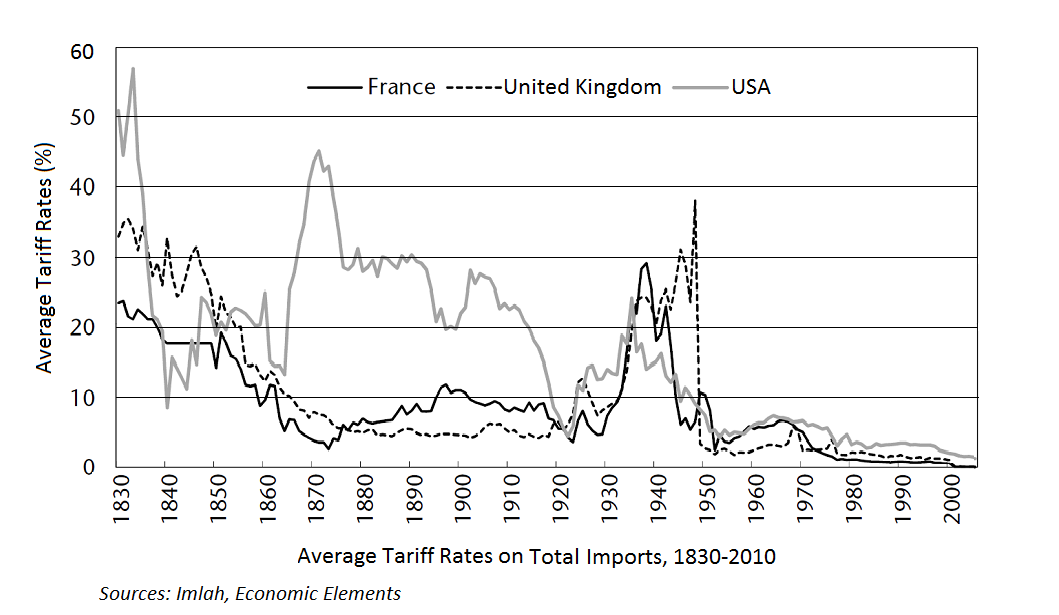
\includegraphics[width=0.7\textwidth]{img/avg_tariff_rates_US_FR_UK.png}
        \caption{Source: Wikipedia based on Albert Imlah's \textquote{Economic Elements}}
        \label{fig:average_tariffs_history}
    \end{figure}
    
    Albeit these tariffs have greatly decreased, many still exist in order to protect some at-risk domestic productions. However, nowadays, countries living in autarky (e.g. self-sufficient) are close to non-existent. Even North-Korea trades goods and services with countries such as Russia or China for instance.
    
    Today, the tariff rates all around the world vary from 0\% to roughly 20\%. A map summarising the average weighted tariff rate applied across all products is presented in Figure~\ref{fig:world_bank_tariffs}. This map is openly available on the World Bank's website\footnote{\url{https://data.worldbank.org/indicator/TM.TAX.MRCH.WM.AR.ZS?end=2018&start=2018&view=map}}.
    
    \begin{figure}[H]
        \centering
        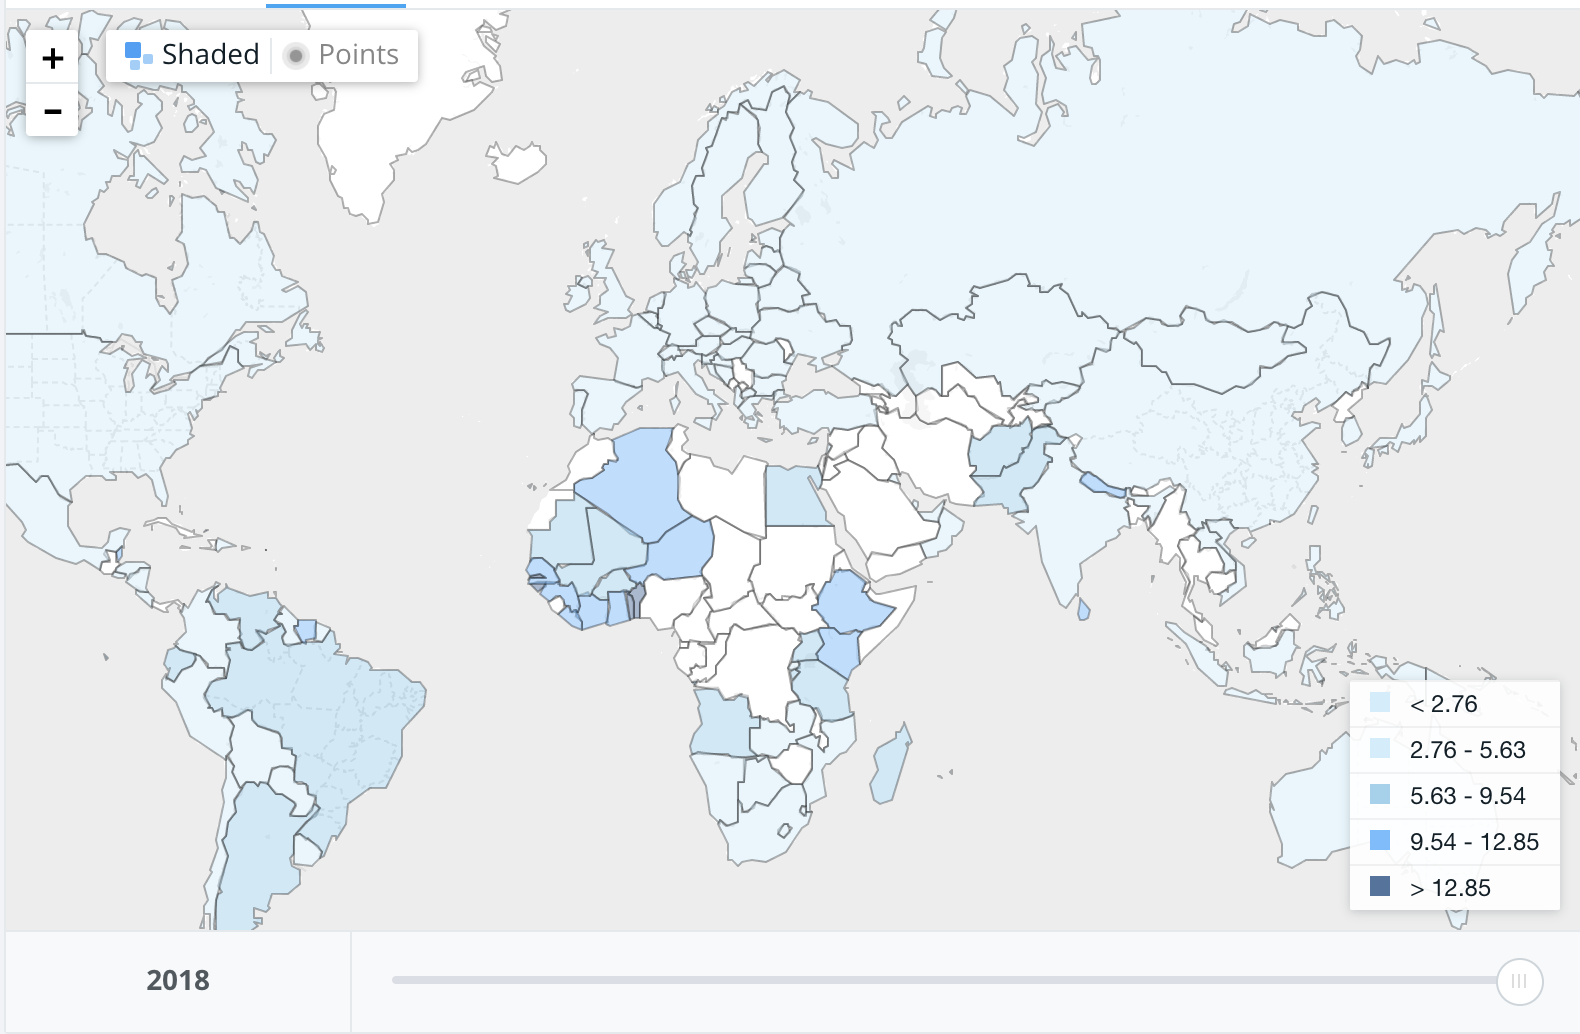
\includegraphics[width=0.7\textwidth]{img/world_bank_tariffs.jpg}
        \caption{Source: World Bank Data}
        \label{fig:world_bank_tariffs}
    \end{figure}
    
    Finally, we will note one very interesting case which is the tariffs rates of small countries, such as remote islands. "The Modern VAT" (\cite{TheModernVAT}) suggests that the advantages of a VAT will be greater than those of a tariff because of the large amount of imports.
    
    
    \subsubsection{Levy (contribution)}
    
    This levy tax can be seen as the income tax in the real world. Nevertheless, the levy tax in our model will be much simpler than the income tax which is a tax based on the income of a year, a time measure which does not exist in our timely discrete World made of ticks.
    
    This tax targets the income and profits earned by an agent, usually during a one-year period. This tax has been around for much longer than the VAT for instance as it appeared in the United Kingdom as early as 1799. In the great majority of the world, this tax is paid by an agent to the State in which it resides. It may be different in some countries (for example in the USA which taxes its citizens, even the non-residents ones), but this particularities go beyond our simulation which only knows the concept of residents.
    
    The income tax can usually be classified in one of the following categories:
    
    \begin{itemize}
        \item Proportional (or flat). In this case, the tax rate is constant across all income levels. The same marginal rate is applied no matter how much income is declared by an agent. Countries applying this kind of taxation include Romania, Russia, or Hungary. Some US states also collect a flat tax (in addition to the federal progressive tax).
        
        \item Progressive. In this case, the tax rate will increase as the income increases (by stages). This is the most used taxation category among the three. As shown by Giacomo Corneo \cite{progressive_taxation}, \textquote{tax progressivity might improve efficiency and the more so in egalitarian  economies}. Indeed, the poorer agents will usually pay a smaller tax rate whereas the richest agents will pay a higher a levy at a higher taxation rate. One should be careful, this is different from a wealth tax which is introduced in the next section~\ref{section:wealth_tax}.
        
        \item Regressive. Contrariwise to the progressive tax, this tax imposes a a greater burden on poorer agents. There are very few examples of such taxation systems.
    \end{itemize}
    
    As usual, the rates will greatly depend from one country to another. Some countries such as the United Arab Emirates do not levy any income tax whereas some countries can collect up to half of the gross income in taxes such Denmark or Belgium.
    
    \subsubsection{Wealth tax}\label{section:wealth_tax}
    
    The wealth tax is a taxation on the assets held by an agent. In our case, we will only take into account the financial assets, and more precisely the money an agent has in its "bank account".
    
    It is, once again, another tool that a State can use to increase its revenues. The idea of a wealth tax is as old as the Ancient Greek civilisation. Indeed, the symmoria \footnote{\url{https://en.wikipedia.org/wiki/Symmoria}} were a group of wealthy citizens that were grouped together with the purpose of collecting a higher tax: a wealth tax to put is simply.
    
    Nowadays, a wealth tax is present in several countries, but it not as generalised at other taxes such as the ones we have previously mentioned. This wealth tax is generally described as a certain percentage of the asset's which has to be paid to the State if the total amount of the assets exceeds a certain threshold. Multiple thresholds can be defined in order to have a progressive wealth tax. For example, taxing 2\% for assets worth more than \$50.000.000 and 6\% for assets worth more than \$1.000.000.000 (1 billion dollars). These are the numbers cited by US senator Elisabeth Warren \footnote{\url{https://www.cbsnews.com/news/elizabeth-warren-wealth-tax-who-would-pay-and-how-much/}}. However, a wealth tax can introduced starting much lower amounts. In Spain for example, the wealth tax starts gradually from 700.000\euro \footnote{\url{https://www.spanishpropertyinsight.com/tax-and-pensions/spanish-wealth-tax-patrimonio/}}.
    
    A huge drawback of the wealth tax is tax evasion and tax havens. Our imperfect simulation will not be able to take these into account unfortunately. According to Åsa Hansson, such a tax could dampen economic growth by reducing the level of investment. However the impact would be very limited.\cite{hansson2010wealth} Again, our imperfect system is not able to model investment and R\&D, therefore, the results in our simulation might be very different.


\subsection{Parameters which the State has direct no leverage on}
    
    As mentioned earlier, there are some key parameters, or rates, which the State cannot influence \emph{directly} contrariwise to the taxes rates. We will dive into two significant rate which have an important role in a economy: the black economy share, and the unemployment rate.

    \subsubsection{Black economy}
    Black economy, also known as shadow economy or non-observed economy \cite{oecdBlack}, is a part of the economy which goes ``unseen'' by the State, usually in order to avoid paying due taxes. One can also note that the formal standardized definition does not include illegal activities (such as drug selling or prostitution) in the black economy share. \cite{pyle1989tax} 
    
    Avoiding paying such taxes allows, on the one hand, the agents to pay less money for their products, therefore being able to buy more products. However, on the other hand, the State will see its taxes revenue decrease hence less money to redistribute later on. 
    If black economy is limited, then its impacts may be negligible. However, if the black economy takes a large part of the total economy, the State will not be able to play its redistribution role resulting eventually in more inequalities among the agents.

    Unfortunately, the black economy is hard to measure precisely. Economists have come up with different kind of methods to evaluate this share such as sampling a portion of the population tax returns and analyze them thoroughly. From this, one can extrapolate the results to a larger scale. \cite{pyle1989tax}. This non-observed economy share has been estimated for several countries, among which some countries of the OECD (Organization for Economic Co-operation and Development) as presented in the figure~\ref{fig:black_economy_oecd} below. It is computed as a share of the total GDP of the country. For instance, Belgium sits at around 22\%. This is a rather significant estimate.
    
    \begin{figure}[H]
        \centering
        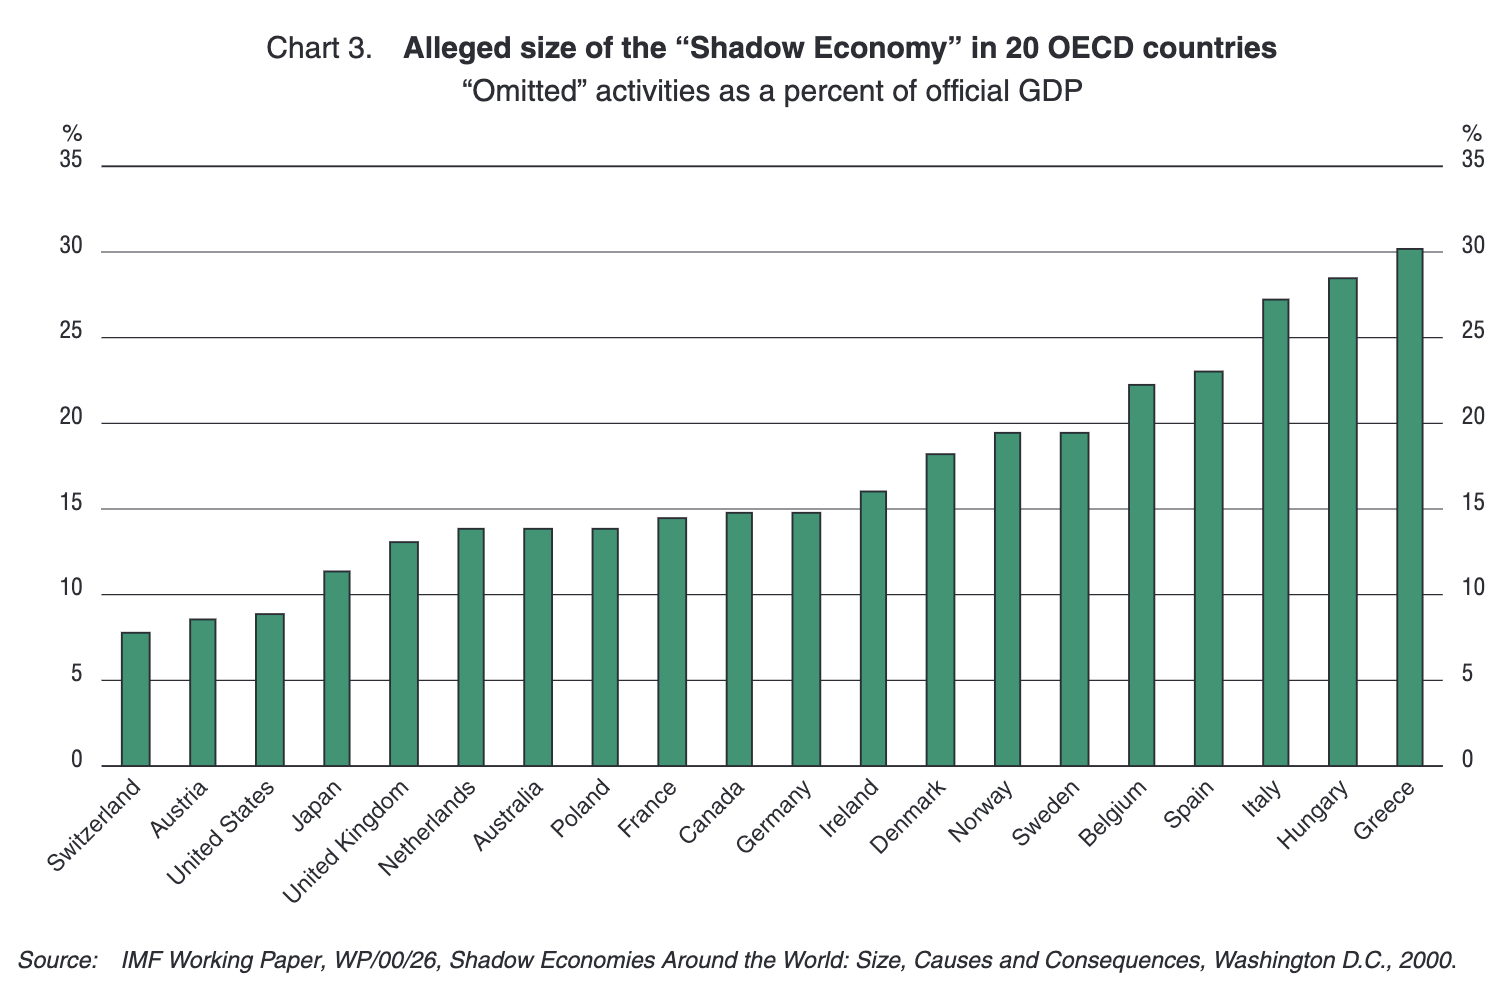
\includegraphics[width=0.8\textwidth]{img/black economy OECD.png}
        \caption{Source: \cite{oecdBlack}}
        \label{fig:black_economy_oecd}
    \end{figure}

    \subsubsection{Unemployment}
    %TODO


\subsection{Allowance and Universal Basic Income}

Because the State has collected money from different taxes, it will now have to redistribute it. In our simulation, there will not be any infrastructure or services that the agents can take advantage of such as public roads or free education. Therefore, all the money levied through taxes will go fully to the wealth distribution system which can be of two types in our system: either through allowances, or through the universal basic income (UBI). It is a exclusive choice, it is either one or the other, not both. So each fictional State will have to make a choice.

    \subsubsection{Allowance}
    
    An allowance is an amount of money given by a State to some of its citizens under certain conditions. The system handling this is called the social security whose role is to provide money to the less fortunate citizens. It insures that every citizen can afford, at least, the most basic needs such as food or shelter. Poorer people will usually receive more money than the wealthier who can already afford a better lifestyle.
    
    However, social security is not always a right in every country. Not all countries have implemented this safety net. According to the United Nations, the majority of the people across the world are not protected by a social security \footnote{\url{https://news.un.org/en/story/2010/11/359142-un-study-finds-most-people-worldwide-have-no-social-security}}. This social security is mostly available in developed countries whereas the percentage of people covered by such a system falls to around 5\% in sub-Saharan Africa.
    
    In our simulation, the social security will be a way of redistributing wealth in order to allow every agent to produce, consume and increase its happiness.
    
    \subsubsection{Universal Basic Income}
    
    Contrariwise to the allowances, in the universal basic income, we give the same amount of money regardless of the situation of each citizen. Everybody receives this amount of money periodically, no strings attached. The idea of a guaranteed income has been proposed throughout history (as early as the 16th century) and some countries have tried it but only for a limited period of time and only for a small sample of the population. Examples of countries that have tried UBI include Kenya, Finland and Macao but at relatively limited scale. 
    
    According to its advocates, the main reason why UBI will be necessary sooner or later is because of the rise of technologies which will replace humans and therefore making them jobless. Its ultimate goal would be to eradicate poverty by assuring everyone a decent amount of money for the most basic needs. And although it might seem Utopian and perhaps not perfect, Thomas Straubhaar, argues that it is worthwhile.\cite{straubhaar2017economics}
    
    However, its detractors critic the cost of such a system and its viability. Another argument is that, although some jobs will be lost, new ones will probably be created; the same way it was done during the industrial revolution. Finally, according to the critics, it is unfair because even the richest people would get this income. Robert Stephens rather suggests \textquote{to simplify and amend the current system, to make it fit  better  with the realities of the 21st century} \cite{stephens2019universal}.

    
\subsection{Economic clusters}
    As we have seen before, countries can impose tariffs on customs in order to discourage imports. However, what if countries had agreements between them in order to allow free trade (thus a null customs tariff) in-between a cluster? The most simple cluster would be made of two States freely importing and exporting from and to one another. This is known as a bilateral agreement. However, we can extrapolate this idea to more countries: a cluster made of a single market where no import tariffs would be levied by its member states.
    
    A very famous real-world example is the European Union (EU). The EU currently counts 27 member states exchanging in one single market with no tariffs on customs. The EU holds lots of advantages among these we can cite a few such as the freedom of movement or worker's protection across all member states, and the most important one being the large common market where goods and services can be exchanged at a cheaper price because of the lack of tariffs which also encourages investment.
    
    It also has some drawbacks such as the membership cost, the non-unique currency, and more bureaucracy. However, these will not be present in our simulation which does not model these aspects.
    
    We should also note that being in a cluster does not exclude a member state from having other bilateral agreements with other states.

\subsection{Efficiency/Equality trade-off}
    Finally, we will briefly discuss the broad question of the efficiency/equality trade-off and why it is a trade-off. Indeed, a trade-off means that improving one side will, generally, deteriorate the other side.
    
    This trade-off has actually been studied in previous works related to this one with the original work being the one of Bersini and van Zeebroeck: \textquote{Why should an economy be competitive ?}. This publication concludes that \textquote{a competitive market distributes welfare much less equally and is responsible for inequality amplifying effect} \cite{bersini}.
    

\section{In computer science}